\documentclass[crop, tikz, border=.1cm]{standalone}
\usetikzlibrary{positioning}
\usetikzlibrary{calc}
\usetikzlibrary{svg.path}
\begin{document}
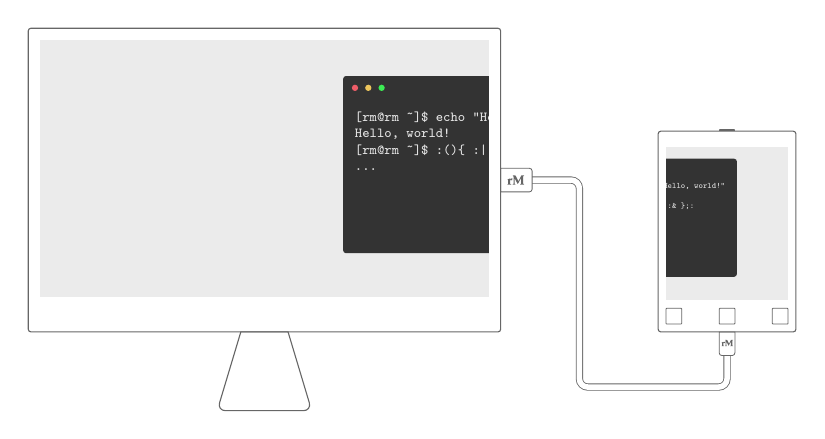
\begin{tikzpicture}
    \colorlet{border}{black!60}
\colorlet{screen}{black!8}
\colorlet{annotation}{black!80}

\newcommand\width{1.75}
\newcommand\height{2.55}
\newcommand\outborder{.1}
\newcommand\button{2 * \outborder}

\newcommand\definehighlightoption[3]{
    \ifcsname Highlight#1\endcsname
        \expandafter\newcommand\csname #1FillColor\endcsname{annotation}
        \expandafter\newcommand\csname #1DrawColor\endcsname{annotation}
    \else
        \expandafter\newcommand\csname #1FillColor\endcsname{#2}
        \expandafter\newcommand\csname #1DrawColor\endcsname{#3}
    \fi
}

\definehighlightoption{UpperKey}{border}{}
\definehighlightoption{HomeKey}{white}{border}

\tikzset{
    secondary/.style={line width=.3},
    back slate/.style={
        border, fill=white,
        rounded corners=1,
    },
    lower key/.style={
        draw=border, secondary, rectangle,
        rounded corners=0.25,
        minimum width={2 * \outborder cm},
        minimum height={2 * \outborder cm},
        inner sep=0pt,
    },
    upper key/.style={
        fill=\UpperKeyFillColor, rectangle,
        rounded corners=0.25,
        minimum width={2 * \outborder cm},
        minimum height=2pt,
        yshift=-.25pt,
        inner sep=0pt,
    },
}

\begin{scope}
    \node[upper key] at (.5 * \width, \height) (key-t) {};
    \draw[back slate] (0, 0) rectangle (\width, \height);

    \fill[screen]
        (\outborder, 4 * \outborder)
        coordinate (screen-bl)
        rectangle (\width - \outborder, \height - 2 * \outborder)
        coordinate (screen-tr);

    \coordinate (screen-c) at ($(screen-bl)!.5!(screen-tr)$);

    \node[lower key] at (2 * \outborder, 2 * \outborder) (key-l) {};
    \node[
        lower key,
        fill=\HomeKeyFillColor,
        draw=\HomeKeyDrawColor
    ] at (.5 * \width, 2 * \outborder) (key-c) {};
    \node[lower key] at (\width - 2 * \outborder, 2 * \outborder) (key-r) {};
\end{scope}


    % Monitor
    \newcommand\monitorwidth{6}
    \newcommand\monitorheight{9*\monitorwidth/14}
    \newcommand\monitorborder{.15}

    \draw[back slate]
        (-8, 0)
        coordinate (monitor-bl)
        rectangle ++(\monitorwidth, \monitorheight)
        coordinate (monitor-tr);

    \fill[screen]
        (monitor-bl) ++(\monitorborder, 3 * \monitorborder)
        coordinate (monitor-screen-bl)
        rectangle ++(
            \monitorwidth - 2 * \monitorborder,
            \monitorheight - 4 * \monitorborder
        )
        coordinate (monitor-screen-tr);

    \path let \p1 = (monitor-tr), \p2 = (monitor-bl) in
        (.5 * \x1 + .5 * \x2, \y2) coordinate (monitor-b);

    \newcommand\supportbase{1.2}
    \newcommand\supportheight{1}
    \newcommand\supporttop{.6}

    \draw[border] (monitor-b)
        -- ++(-.5 * \supporttop, 0)
        {[rounded corners=3]
        -- ++({-.5 * (\supportbase - \supporttop)}, -\supportheight)
        -- ++(\supportbase, 0)}
        -- ++({-.5 * (\supportbase - \supporttop)}, \supportheight)
        -- cycle;

    % Cable
    \newcommand\logo{
        svg "m0,0c1.21644,-1.76175,2.369961,-3.20889,3.460563,-4.34144c1.132547,-1.17449,2.013418,-1.76174,2.642611,-1.76174c0.880871,0,1.82466,0.14681,2.831369,0.44044c1.006709,0.25167,1.719795,0.4614,2.139257,0.62919l-2.642611,7.92783c-0.503355,-0.29362,-1.27936,-0.65016,-2.328015,-1.06962c-1.006709,-0.46141,-1.992445,-0.69212,-2.957208,-0.69212c-1.258386,0,-2.307041,0.37752,-3.145966,1.13255v15.85567l5.473981,3.39764v0.37752h-17.492v-0.37752l3.523482,-3.20888v-16.04443l-3.397643,-2.70553v-0.37752l11.891751,-5.34814z"
        svg "m59.332919,23.9178l4.467272,3.901v0.37752h-18.75v-0.37752l4.530191,-3.901v-25.79692l-14.534363,27.11823h-0.94379l-14.157,-26.992v25.67108l4.467272,3.901v0.37752h-13.087v-0.37752l4.467271,-3.901v-31.523c-0.08389,-0.12584,-0.314596,-0.46141,-0.692112,-1.00671c-0.377516,-0.58725,-0.796978,-1.19547,-1.258387,-1.82466c-0.419462,-0.67114,-0.817951,-1.27936,-1.195467,-1.82466c-0.377516,-0.5453,-0.587247,-0.8599,-0.629193,-0.94379v-0.25168h12.080509l13.590573,25.79692l13.401815,-25.79692h12.583863v0.25168l-4.341432,4.02683z"
    }

    \path (.5 * \width, 0) coordinate (device-port);
    \path (monitor-tr) ++(0, -.5 * \monitorheight) coordinate (monitor-port);

    \draw[
        border, rounded corners=3,
        double, double distance=2,
        secondary
    ]
        (monitor-port) ++(.4, 0)
        let \p1 = (monitor-tr) in -| (.5 * \x1, 0)
        |- ($(device-port)+(0, -.7)$)
        -- ++(0, .4);

    \draw[border, secondary]
        (device-port) ++(-.1, 0)
        -- ++(.2, 0) {[rounded corners=1]
        -- ++(0, -.3)
        -- ++(-.2, 0)}
        -- cycle;

    \begin{scope}[xscale=.055, yscale=-.055]
        \fill[border] (device-port) ++(-.85, 2.5) \logo;
    \end{scope}

    \draw[border, secondary]
        (monitor-port) ++(0, .15)
        {[rounded corners=1]
        -- ++(.4, 0)
        -- ++(0, -.3)}
        -- ++(-.4, 0)
        -- cycle;

    \begin{scope}[xscale=.08, yscale=-.08]
        \fill[border] (monitor-port) ++(1.5, -.05) \logo;
    \end{scope}

    % Window
    \newcommand{\windowcontents}{
        \detokenize{[rm@rm ~]$ echo "Hello, world!"}\\
        Hello, world!\\
        \detokenize{[rm@rm ~]$ :(){ :|:& };:}\\
        ...
    }

    \begin{scope}[shift={(-4, 1)}]
        \clip (monitor-screen-bl) rectangle (monitor-screen-tr);
        \fill[annotation, rounded corners=1] (0, 0) rectangle ++(3, 2.25);

        \definecolor{button-red}{HTML}{EE5D68}
        \definecolor{button-yellow}{HTML}{ECC55C}
        \definecolor{button-green}{HTML}{3CEB54}

        \tikzset{
            button/.style={
                circle,
                inner sep=0pt,
                minimum width=.08cm
            },
            button red/.style={button, fill=button-red},
            button yellow/.style={button, fill=button-yellow},
            button green/.style={button, fill=button-green},
        }

        \node[button red] at (\monitorborder, 2.25 - \monitorborder) (red) {};
        \node[button yellow, right=.5 * \monitorborder of red] (yellow) {};
        \node[button green, right=.5 * \monitorborder of yellow] (green) {};

        \node[
            align=left,
            font=\ttfamily\tiny\color{black!10},
            anchor=north west,
            inner sep=0pt,
            outer sep=0pt,
        ] at (\monitorborder, 2.25 - 3 * \monitorborder) {\windowcontents};
    \end{scope}

    \begin{scope}[shift={(-1, .7)}]
        \clip (screen-bl) rectangle (screen-tr);
        \fill[annotation, rounded corners=1] (0, 0) rectangle ++(2, 1.5);

        \node[
            align=left,
            font=\ttfamily\tiny\color{black!10},
            anchor=north east,
            inner sep=0pt,
            outer sep=0pt,
            scale=.6,
        ] at (2 - \monitorborder, 1.5 - 2 * \monitorborder) {\windowcontents};
    \end{scope}
\end{tikzpicture}
\end{document}
